\documentclass[a4paper,12pt,fullpage]{article}



\usepackage[paperwidth=19cm,paperheight=25.7cm,hmargin=2cm, vmargin=2cm]{geometry}
\usepackage[a4,frame,center,noinfo]{crop}
\usepackage{array}
\usepackage{subfiles}


\usepackage{supertabular}
\usepackage{float}
\usepackage[section]{placeins}

\usepackage{tocloft}
\renewcommand{\cftsecleader}{\cftdotfill{\cftdotsep}} % for sections




\usepackage{hyperref}
\hypersetup{
	colorlinks=true,
	linkcolor=blue,
	filecolor=magenta,      
	urlcolor=cyan,
	citecolor=cyan
}


\usepackage{xepersian}
\settextfont{XB Niloofar}
\setlatintextfont[Scale=0.85]{Times New Roman}



\title{تسک دیجی شهر}

\author{شایان صادقی}
\begin{document}
	
	\pagenumbering{alph}
	\maketitle
	\pagebreak
	
	\pagenumbering{arabic}
	
	\section{بخش اول}
	در این بخش نیاز به اجرای چند کوئری به زبان \lr{sql} وجود داشت. از طرفی فایل داده‌های موجود با پسوند \lr{.db} ارائه شده بودند. بنابراین برای دسترسی به محتویات دیتابیس \lr{sqlite} از یک ابزار کلاینت دیتابیس مناسب مانند \lr{dbeaver} استفاده شد.
	
	\subsection{سوال ۱}
	کوئری مربوطه در شکل \ref{fig1_1} و نتایج در شکل \ref{fig1_1_res} نشان داده شده است. در بررسی اولیه داده‌ها، وجود دو واحد پول مشخص شد که برای همین منظور لازم است مقدار \lr{sales} در داده‌ها یکسان شود. مقدار تبدیل نشده برای مقایسه در ستونی مجزا مشخص شده است. با توجه به رکورد ردیف ۴ می‌توان تأثیر بی‌توجهی به نرخ تبدیل ارز را مشاهده کرد.
	
	\begin{figure}[hbt!]
		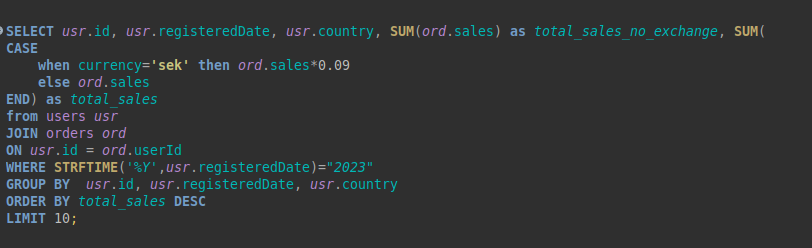
\includegraphics[width=\linewidth]{"./images/q1.1.png"}
			\caption{کوئری ۱}
		\label{fig1_1}
	
	\end{figure}

\begin{figure}[hbt!]
	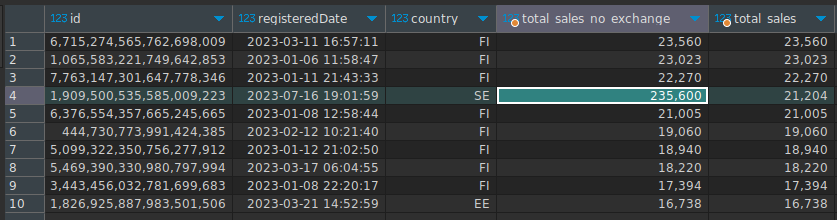
\includegraphics[width=\linewidth]{"./images/q1.1_res.png"}	
	\caption{۱۰ کاربر با بیشترین مقدار \lr{sales} در سال ۲۰۲۳}
	\label{fig1_1_res}
	
\end{figure}


\subsection{سوال ۲}
برای مشخص کردن بیشترین سفارش ثبت شده از اتصال نتایج دو جدول \lr{orders} و  \lr{providers} استفاده شده است. مطابق کوئری شکل \ref{fig1_2} بیشترین سفارش ثبت شده مربوط به خرید وعده غذایی با تعداد 305,254 می‌باشد.


\begin{figure}[hbt!]
	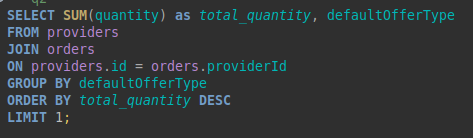
\includegraphics[width=\linewidth]{"./images/q1.2.png"}
	\caption{کوئری 1-2}
		\label{fig1_2}
\end{figure}

\section{بخش دوم}
در ادامه این بخش لازم است فایل \lr{csv} تعطیلات را در دیتابیس فعلی باز کرده تا دسترسی لازم به همه دیتاها ایجاد شود.

\subsection{سوال ۱}
به کمک کوئری شکل \ref{fig2_1} و نتایج به دست آمده که در شکل \ref{fig_2_1_res} نشان داده شده است. یکی از دلایل احتمالی، سفر مردم به خارج از شهر و در نتیجه عدم استفاده از این اپلیکیشن است. همچنین ممکن است به دلیل حضور مردم در خانه -و نه در محل کار- فرصت کافی برای پخت غذا توسط خودشان در روزهای تعطیل وجود داشته باشد.
\begin{figure}[hbt!]
	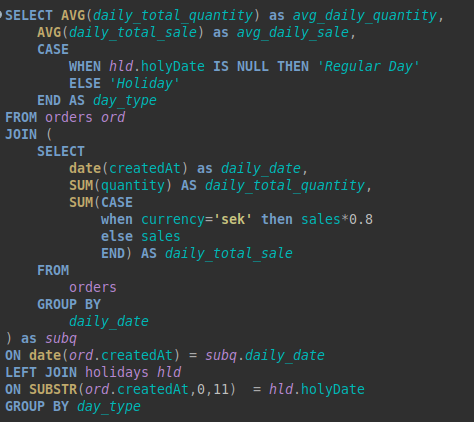
\includegraphics[width=\linewidth]{"./images/q2.1.png"}
	\caption{کوئری 2-1}
	\label{fig2_1}
\end{figure}

\begin{figure}[hbt!]
	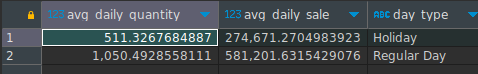
\includegraphics[width=\linewidth]{"./images/q2.1_res.png"}
	\caption{میانگین مجموع تعداد و درآمد فروش روزانه در تعطیلات و روز‌های عادی}
	\label{fig_2_1_res}
\end{figure}

\subsection{سوال ۲}
با توجه به نتایج به دست آمده، تعداد تأمین‌کنندگان نیز در روزهای تعطیل کاهش یافته است. در این کوئری تعداد روزهای تعطیل و غیرتعطیل نشان داده شده است. تفاوت تعداد نمونه‌های این دو دسته می‌تواند منجر به تفاوت واریانس دو نمونه و نقض شرط برابری واریانس نمونه‌ها شود. بنابراین بهتر است در صورت نیاز به انجام آزمون فرض آماری برای بررسی معناداری، از آزمون‌های غیر پارامتری استفاده شود. 

علت احتمالی کاهش تأمین‌کنندگان در روزهای تعطیل را می‌توان مرتبط با کاهش تقاضای کاربران در این روز‌ها دانست.
\begin{figure}[hbt!]
	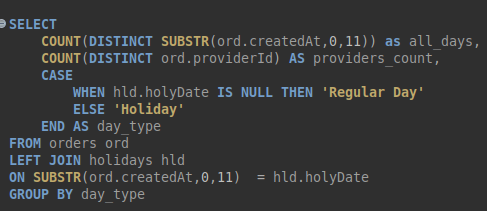
\includegraphics[width=\linewidth]{"./images/q2.2.png"}
	\caption{کوئری 2-2}
	\label{fig2_2}
\end{figure}

\begin{figure}[hbt!]
	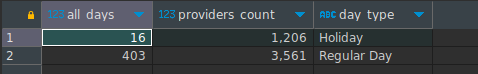
\includegraphics[width=\linewidth]{"./images/q2.2_res.png"}
	\caption{تعداد تأمین‌کنندگان به تفکیک روزهای عادی و تعطیلات}
	\label{fig2_2_res}
\end{figure}


\subsection{سوال ۳}
با توجه به نتایج قسمت‌های قبل به نظر می‌رسد این کمپین موفقیت‌آمیز نبوده است.	

\section{بخش سوم}
داشبورد مورد نظر در شکل \ref{fig_dash} نشان داده شده است. برای محاسبه \lr{m1 retention} از کد پایتون نیز کمک گرفته شده است که در شاخه \lr{python\_files} قرار دارند.

\begin{figure}[hbt!]
	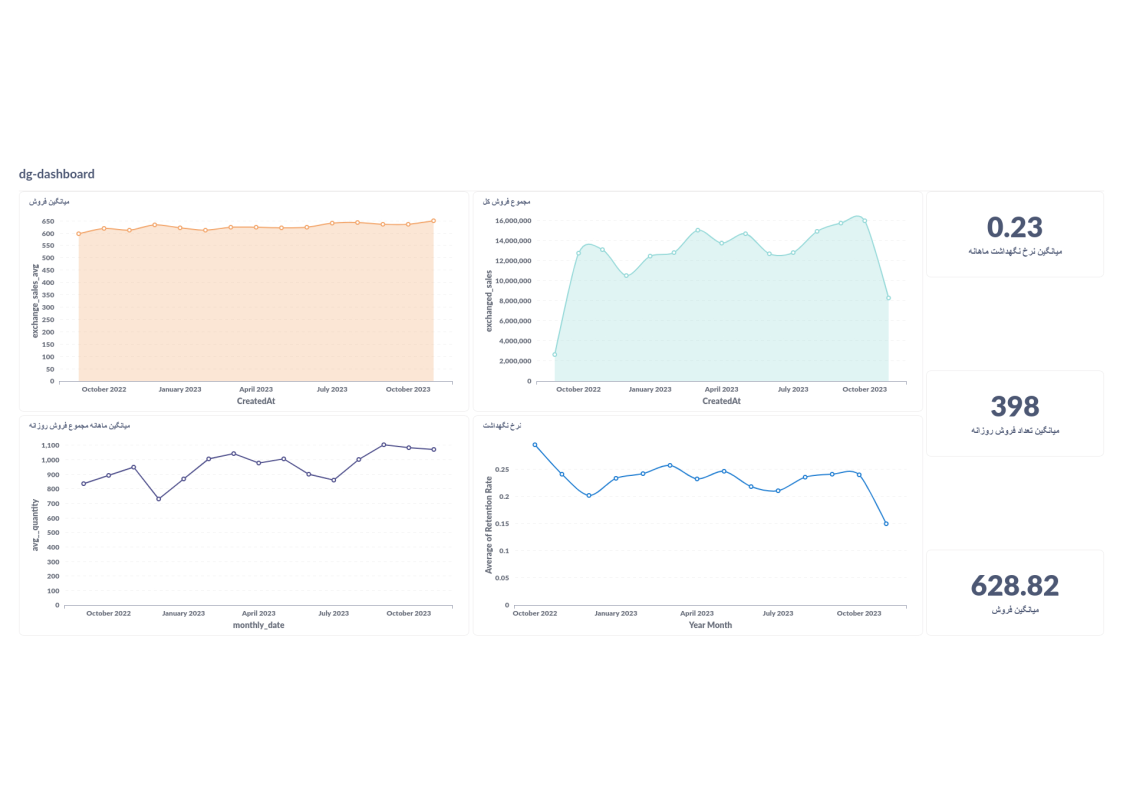
\includegraphics[width=\linewidth]{"./images/dashboard.png"}
	\caption{داشبورد}
	\label{fig_dash}
\end{figure}

\end{document}